\section{On-accelerator training framework} \label{sec:framework}
In contrast to the typical offline training framework on GPPs, we propose an 
on-accelerator training framework to allow the CNN accelerator's runtime variation 
to be learned with the application data. It targets a CPU + CNN accelerator platform 
while we
to take these accelerators’ dynamic behaviors into consideration during training 
to tolerate the ‘un-deterministic’ behavior of the ‘unstable’ accelerators. The basic 
idea is to embed the CNN accelerator into the conventional training framework so that 
the accelerator is referenced during training. In this work, we choose Caffe as the baseline 
training framework because it is more natural to integrate the C/C++ based high 
level synthesis CNN accelerator. Based on Caffe, we further detail the required general 
interface to make use of the hardware accelerator in training, and introduce 
the necessary modifications to the CNN accelerator structure. 

  
  In contrast to the conventional off-line training on CPUs and GPUs, we propose 
to take these accelerators’ dynamic behaviors into consideration during training 
to tolerate the ‘un-deterministic’ behavior of the ‘unstable’ accelerators. The basic 
idea is to embed the CNN accelerator into the conventional training framework so that 
the accelerator is referenced during training. In this work, we choose Caffe as the baseline 
training framework because it is more natural to integrate the C/C++ based high 
level synthesis CNN accelerator. Based on Caffe, we further detail the required general 
interface to make use of the hardware accelerator in training, and introduce 
the necessary modifications to the CNN accelerator structure. 
\subsection{Proposed Training Framework }
  Figure 3 illustrates the proposed training framework. It begins with the 
off-line training result which can greatly shorten the overall training time. 
While most of the CNN accelerator adopts fixed point operations, the pre-trained model 
is therefore expected to be fixed point model. With the pre-trained model, 
we mainly try to have the trained model to further adapt to the ‘un-deterministic’ 
behaviors which are difficult to model on CPUs and GPUs.

\begin{figure*}
        \center{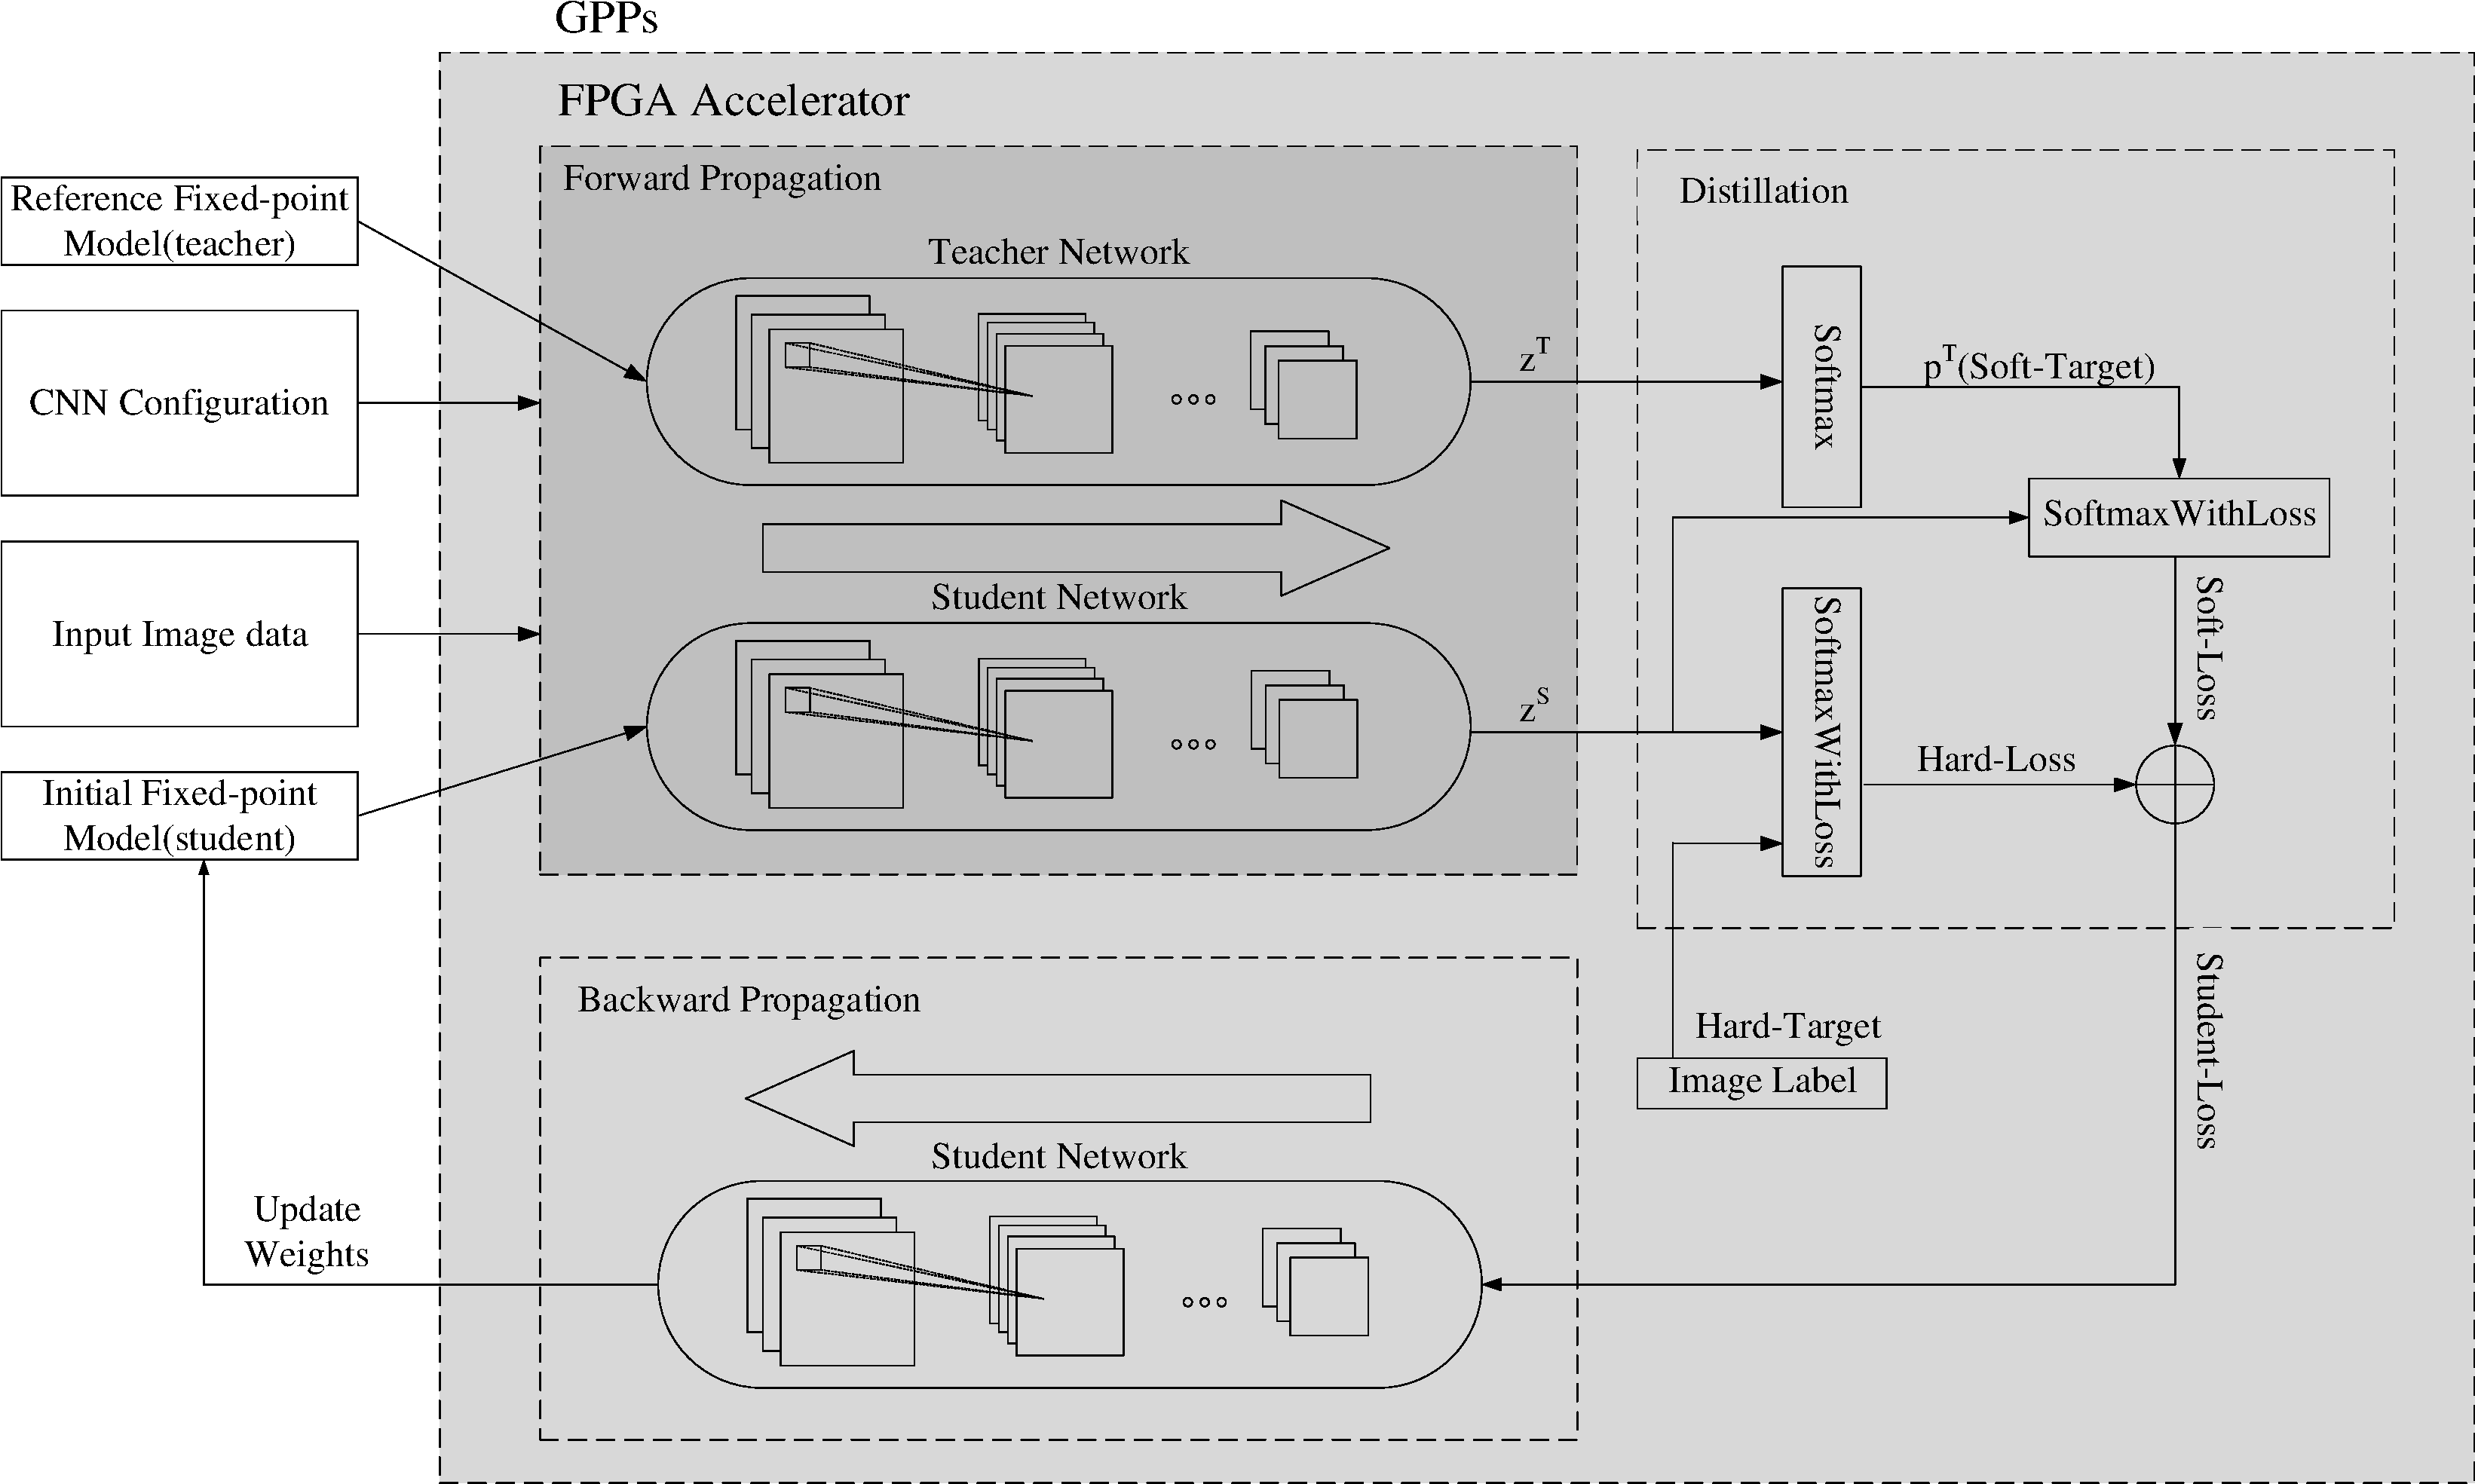
\includegraphics[width=0.85\linewidth]{retrain}}
        \caption{Training Framework}
        \label{fig:retrain}
%        \vspace{-0.5em}
\end{figure*}


  To that end, we have the forward propagation performed on the accelerator 
directly while the backward propagation remains on CPUs or GPUs. Forward propagation 
on the accelerator is fixed point, which is beneficial to both the resource consumption 
and memory bandwidth overhead, but backward propagation on CPUs or GPUs remains floating 
point to ensure the small changes in the parameters get accumulated\cite{Matthieu2014_8}. As a result, 
we still need additional converting between the fixed point and floating during 
the training in each iteration when the weight is adjusted. When the final accuracy 
loss reaches the threshold, it means that the model can tolerate 
the accelerator’s ‘un-deterministic’ behaviors. And the CNN model can be safely 
deployed on the ‘unstable’ accelerator. 

Figure 4 depicts the implementation of the training framework on a hybrid 
CPU-FPGA architecture. In this work, we use Xilinx KCU1500 as the FPGA board 
and put it on a standard desktop computer. CPU is the controller and it reconfigures 
the accelerator for a specific CNN structure. In each training iteration, CPU launches 
the CNN accelerator to perform the forward propagation from bottom layer to top layer. 
CPU does the backward propagation from top layer to bottom layer. Weights and the image 
data are initially stored in host memory. It will be transferred to FPGA offchip memory 
for forward propagation through PCI-E. Similarly, the output data will be transferred 
from FPGA off-chip memory back to host memory after forward propagation. Because of the 
OpenCL based API wrapper in SDAccel, the CNN accelerator’s interface can be easily 
exposed to Caffe for referring to the forward propagation result. 

%\begin{figure}
%        \center{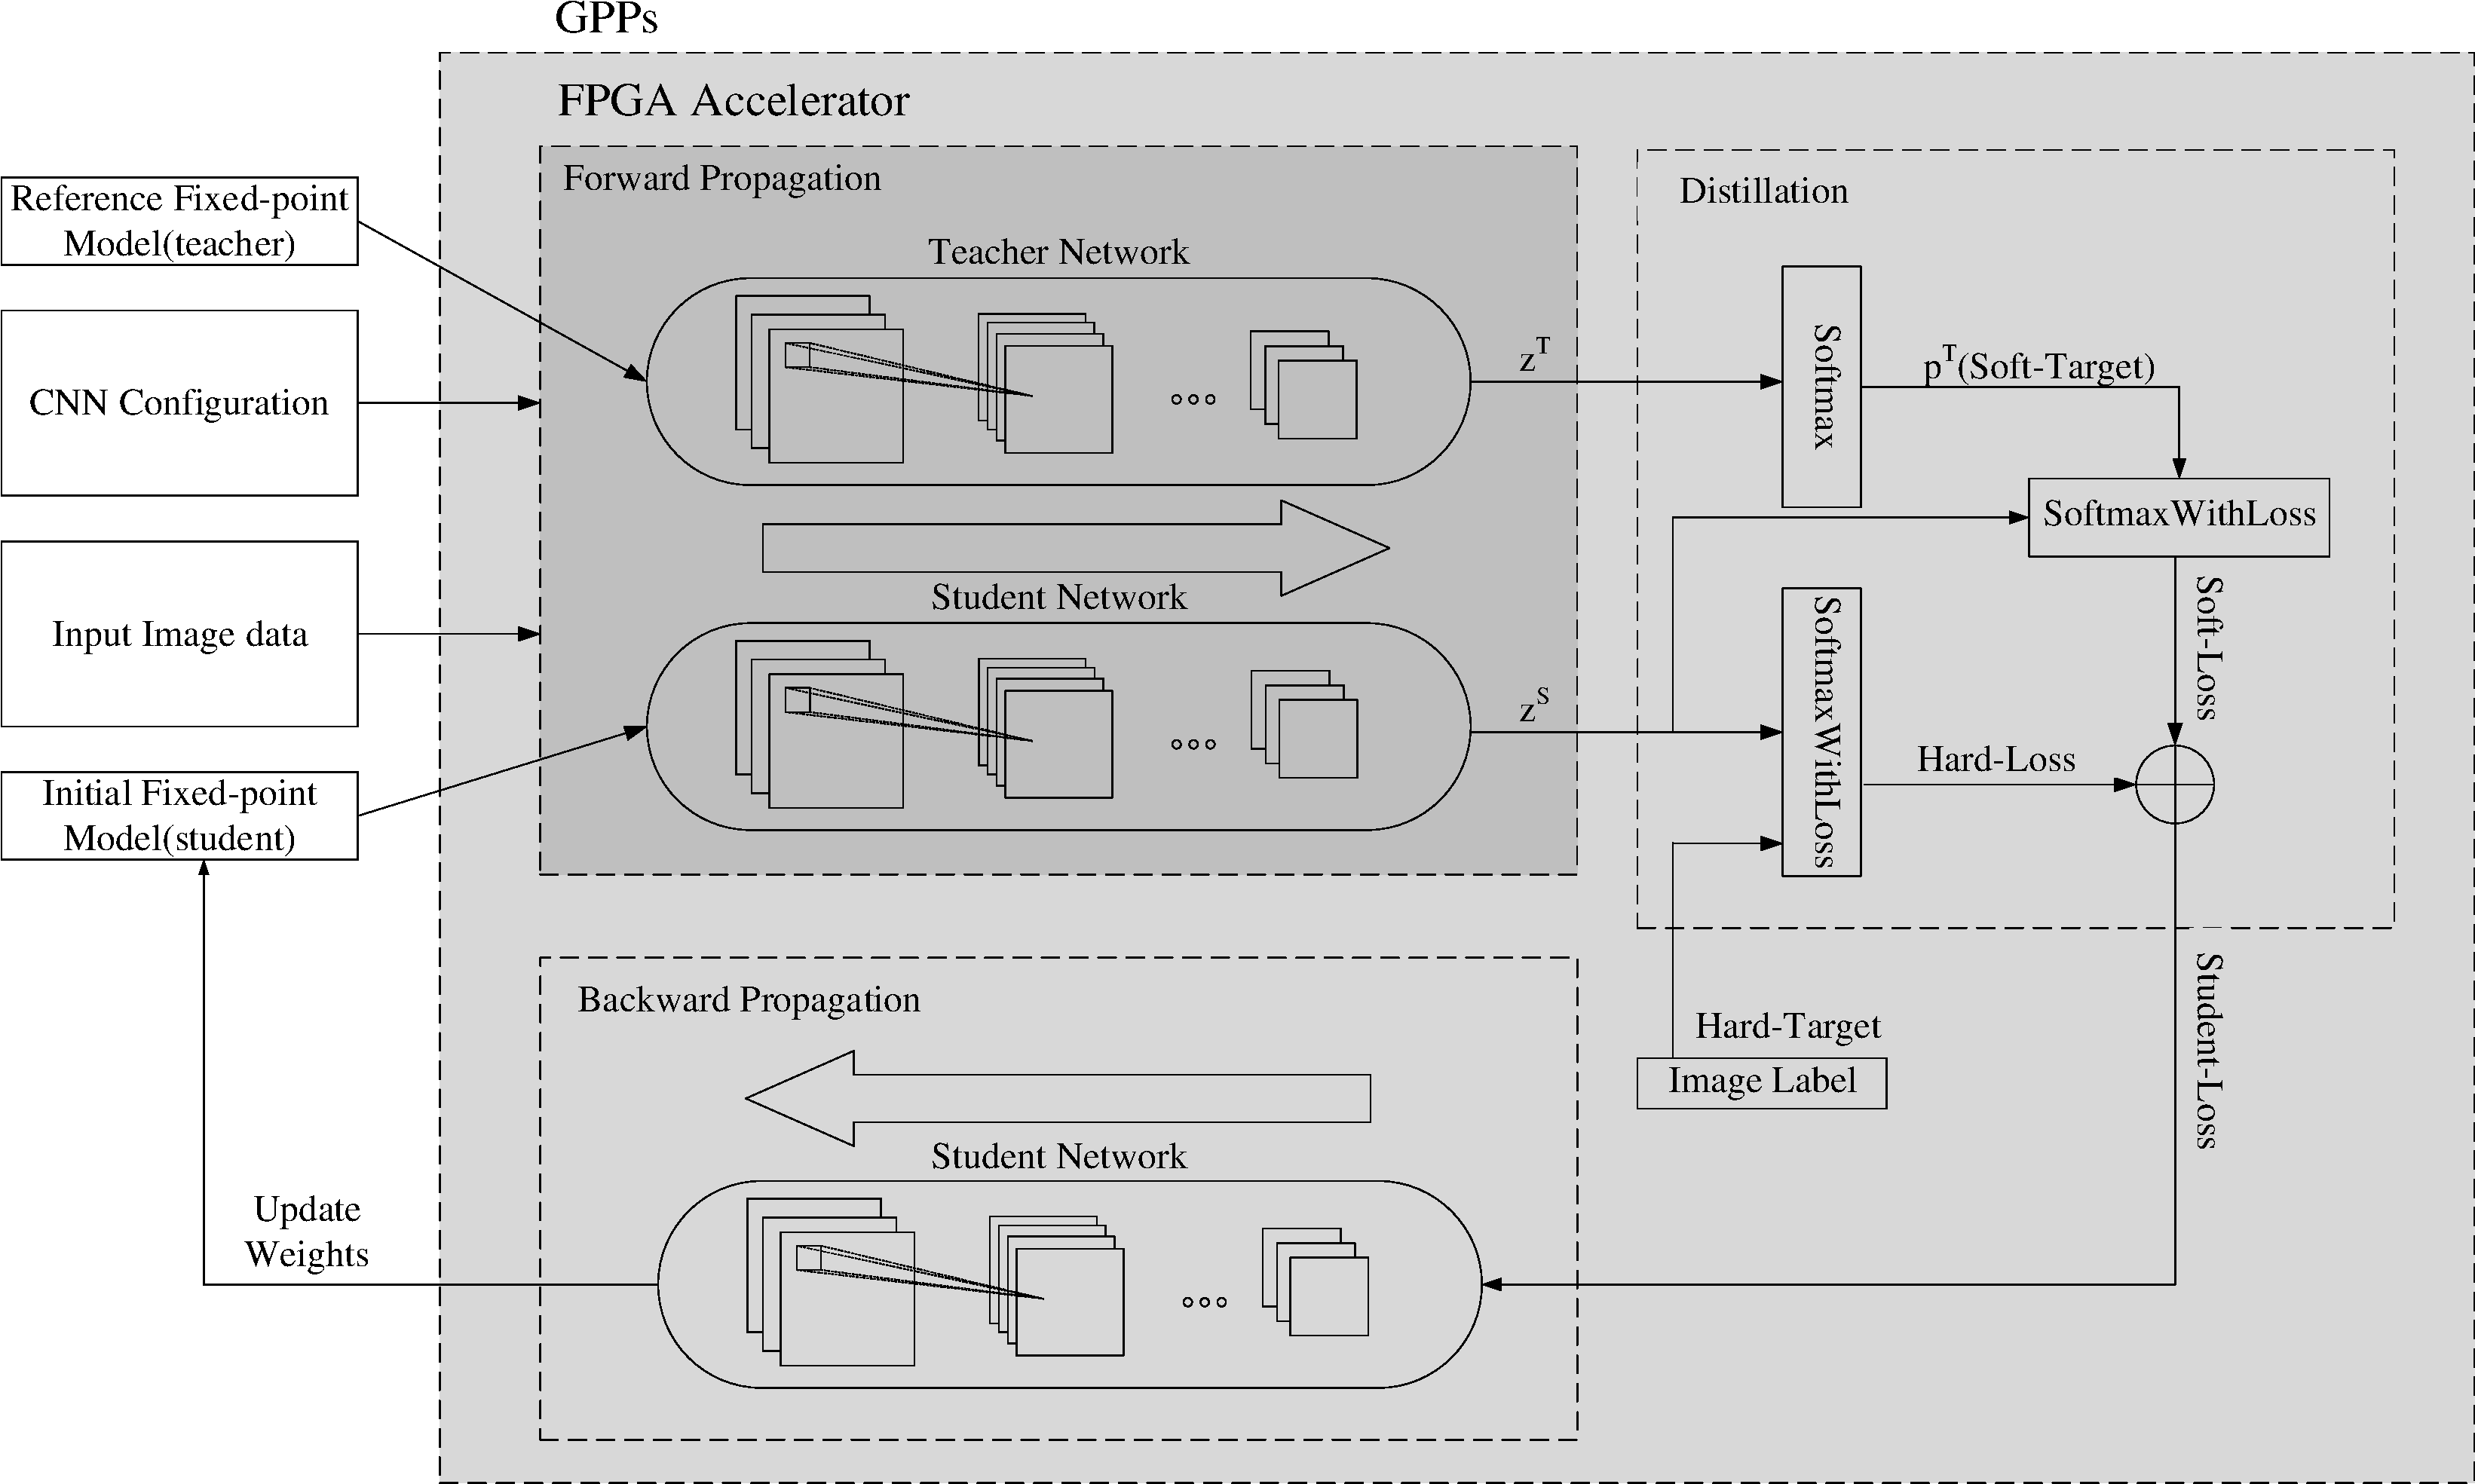
\includegraphics[width=0.85\linewidth]{retrain}}
%        \caption{Training on Hybrid CPU-FPGA Architecture}
%        \label{fig:framework}
%        \vspace{-1em}
%\end{figure}


\subsection{High Level Accelerator Interface to Caffe }
  With the growing popularity of deep learning, massive different 
CNN accelerators have been developed over the years. In order to fit various CNN accelerators 
within the same training framework, we define a set of high-level interface functions as listed 
in Table 1. There are 7 functions included. Function 1 is used to launch the CNN accelerator from host. 
Function 2 and 3 are used to transfer data between the host memory and the device memory during 
the training. As most of the accelerators are fixed point and used for forward while back propagation 
is floating point, Function 4 and 5 are required for training when forward and backward 
propagation are iteratively committed. Function 1 to 5 are required for all the accelerators. 
Function 6 and 7 are only needed for accelerators that perform on reorganized data\cite{pipecnn_2,deepburing_12}. 
With the interface functions, general CNN accelerators can be trained to tolerate ‘un-deterministic’ circuit 
behaviors using the proposed framework.
  CNN accelerators can either be implemented using high-level synthesis tools (HLS) or hardware description 
languages (HDL). With Xilinx SDAccel, we can wrap the both types of accelerators with OpenCL API. 
With the OpenCL API, Caffe can refer to the accelerators during training conveniently. 

\begin{table*}
        \centering
        \vspace{-0.3em}
        \caption{High-level interface to integrate general CNN accelerators with Caffe}
        \label{tab:graph}
        \vspace{-0.3em}
        \begin{tabular}{c|l|l}
                \toprule
                ID & Function Name & Description  \\
                \midrule
                1 & launchAccelerator() & It configures the CNN accelerator and launches it from host CPU. \\
		\midrule
                2 & dataToFPGA(weight, input, wgtDevAddr, inDevAddr) & It transfers both the input data and weight to the FPGA device memory. \\
		\midrule
		3 & dataFromFPGA(outputDevAddr, output) & \shortstack[l]{It transfers all the intermediate output of the CNN layers from FPGA \\device memory to host memory.} \\
		\midrule
		4 & convertIntToFloat(int iData, float fData) & It converts the fixed-point output to float for back propagation processing. \\
		\midrule
		5 & convertFloatToInt(float fData,  int iData) & \shortstack[l]{It converts the floating-point input and weight data to fixed point or \\integer for forward processing on the accelerator.} \\
		\midrule
		6 & dataLayoutReorder(data, reorderedData) & \shortstack[l]{It reorders the data layout for more efficient accelerator execution before \\sending to FPGA device memory.} \\
		\midrule
		7 & dataLayoutRecover(reorderedData, data) & It reorders the output data back to the default format for Caffe back propagation. \\
                \bottomrule
        \end{tabular}
        \vspace{-1em}
\end{table*}

\subsection{Modification to the general CNN accelerators}
  On top of the interface, the CNN accelerator also needs minor adjustment for the training. 
The training process requires the feature maps of each CNN layer for backward propagation, 
while the accelerators are typically optimized for inference and some of the layers’ output 
are fully buffered in on-chip memory for less memory access overhead. In this case, 
the accelerator should make intermediate output write back optional as shown in Figure 5. 
When the accelerator is used in training, the output will be transferred to memory. 
When it is used for inference, it can also turn off the write back data path for better performance. 
It is trivial to modify the CNN accelerators and the hardware overhead is negligible.

\begin{figure}
        \center{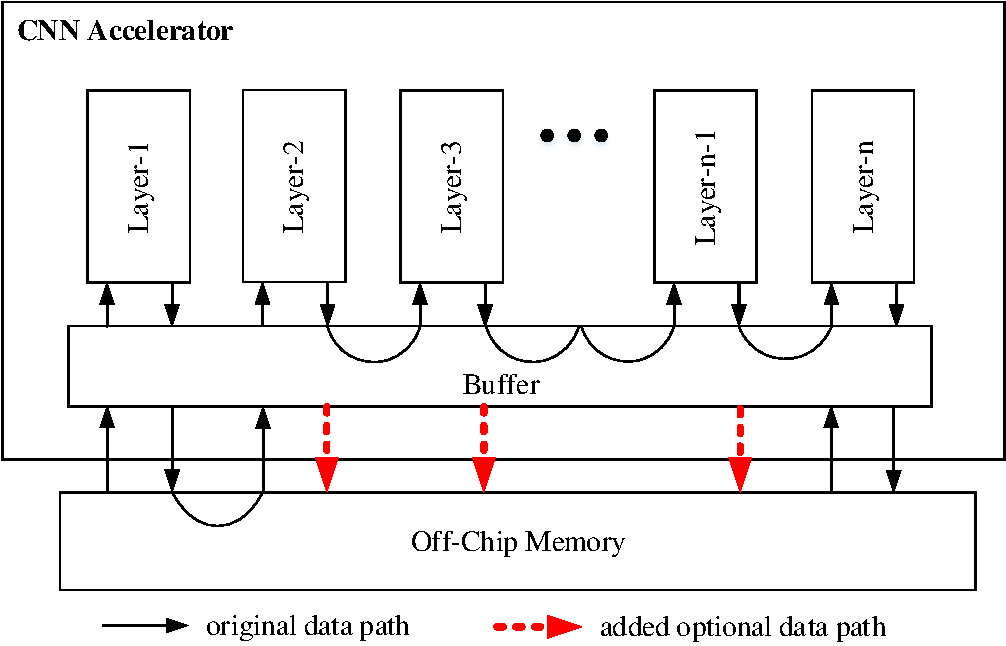
\includegraphics[width=0.85\linewidth]{change_of_accelerator}}
        \caption{Modification of the CNN accelerator data path. It essentially
ensures each CNN layer to have an optional data path to off-chip memory so that it
can be used for training as necessary.}
        \label{fig:change_of_accelerator}
        \vspace{-1em}
\end{figure}


